\documentclass[a4paper]{article}
\usepackage[cm]{fullpage}
\usepackage{standalone}
\usepackage[utf8]{inputenc}
\usepackage[british]{babel}
\usepackage{csquotes}
\usepackage[T1]{fontenc}
\usepackage{charter}
\usepackage[bitstream-charter]{mathdesign}
\usepackage{natbib}
\usepackage[final,babel]{microtype}
\usepackage[hidelinks]{hyperref}
\usepackage{siunitx}
\usepackage[margin=3pt]{subcaption}
\usepackage{xcolor}
\PassOptionsToPackage{final}{graphicx}
\usepackage{tikz}
\usetikzlibrary{arrows}
\usetikzlibrary{patterns}
\usepackage{bm}

\title{Monitoring Committee Progress Report \#2\\
\vspace*{1em}
\Large{Numerical Representation of Mountains in Atmospheric Models}}
\author{James Shaw
\vspace{0.5em} \\
\large{Supervisors: Hilary Weller, John Methven, Terry Davies}
\vspace{0.5em} \\
\large{Monitoring Committee: Maarten Ambaum, Paul Williams}}
\date{3rd December 2015}

\makeatletter
\AtBeginDocument{
  \hypersetup{
    pdftitle = {Monitoring Committee Progress Report \#2},
    pdfauthor = {James Shaw}
  }
}
\makeatother


\begin{document}
\newcommand{\exner}{\Pi}
\maketitle


I am reaching the end of the first year of my PhD, having started in January 2015.
The PhD aims to find ways of improving the accuracy of dynamical cores in the presence of orography.
Most of my research so far has involved comparing numerical accuracy between terrain following and cut cell grids.
At the time of our last monitoring committee meeting in June 2015, Hilary and I had documented our findings and submitted a manuscript to Monthly Weather Review.  A key result was that thermal errors were present on the cut cell grid in a two-dimensional mountain waves test.  Following reviewer comments, we have performed additional tests to establish that the thermal errors are caused by errors in the advection of potential temperature.  We submitted a revised manuscript in October 2015.

The new test results also prompted us to improve the advection scheme so that it remains upwind-biased even when the downwind cell is very small.  Combined with a novel grid generation technique, this offers a new approach for avoiding the `small cell problem' associated with explicit numerical schemes on cut cell grids.  We intend to describe the advection scheme and the cut cell grid generation technique in a new publication.

We also wish to develop a Charney--Phillips staggering for arbitrary grids.  There is no existing formulation for such grids, and the first monitoring committee report identified this as an area for future work.  We have since made some preliminary progress, having implemented a new formulation in a finite volume model, but more testing is required to verify correctness and assess the accuracy of the scheme.  Later on, we expect to develop Eulerian thermal advection schemes for this new type of grid.

In November 2015 I attended the GungHo workshop at the Met Office.  GungHo is a project to develop a new numerical weather prediction model, which includes a new dynamical core named Dynamo.  I have spoken with Met Office scientists about how my research might benefit this project, and they are particularly interested in our work on Charney--Phillips Eulerian advection schemes.

\section{Comparison of terrain following and cut cell grids}
Terrain has an impact on all scales of atmospheric flow, generating planetary waves and gravity waves, retarding frontal systems, and forcing flow through channels and along slopes and valleys.  Extreme weather can be induced by flow over mountains, creating downslope windstorms and affecting local precipitation.  An accurate representation of orography is necessary to model these processes correctly.

Terrain following (TF) layers are the most common way to represent orography, in which the lowest model layers follow the terrain, while layers are gradually flattened with increasing height.  There are several choices of decay function that govern how layers are flattened aloft, and our experiments use two: the Basic Terrain Following (BTF) coordinate \citep{galchen-somerville1975}, and the Smooth LEvel VErtical (SLEVE) coordinate \citep{schaer2002}, examples of which are shown in figures~\ref{fig:btf} and \ref{fig:sleve} respectively.  TF layers are attractive because their rectangular structure is simple to process by computer and link with parametrizations, and boundary layer resolution can be increased with variable spacing of vertical layers \citep{schaer2002}.
However, increasing horizontal resolution can lead to steeper slopes and more non-orthogonal grids which reduce the accuracy of pressure gradient calculations and can generate spurious circulations \citep{dempsey-davis1998,klemp2011}.

\begin{figure}
	\centering
	\footnotesize
	\subcaptionbox{Basic terrain following (BTF) grid \label{fig:btf}}[.3\linewidth]{\input{../fig-grids/btf}}
	\subcaptionbox{Smooth level vertical (SLEVE) grid \label{fig:sleve}}[.3\linewidth]{\input{../fig-grids/sleve}}
	\subcaptionbox{Cut cell grid.  Small cells are marked by an asterisk ($\ast$). \label{fig:cutCell}}[.3\linewidth]{\input{../fig-grids/cut-cell}}
%
	\caption{Examples of levels in BTF and SLEVE terrain following grids and a cut cell grid.}
	\label{fig:grids}
\end{figure}

The cut cell method is an alternative to TF layers in which the terrain is intersected with a rectangular, orthogonal grid.  Cells below the surface are removed and cells that are intersected by the terrain are `cut', modifying their shape and size \citep{adcroft1997}.  Cut cell grids reduce errors in calculating pressure gradients because they are more orthogonal than equivalent terrain following grids, but the cut cell method can create some very small cells that constrain the timestep for explicit advection schemes \citep{klein2009}.  Figure~\ref{fig:cutCell} shows an example cut cell grid with small cells indicated by asterisks.

\subsection{Results}
We used a finite volume model of the fully-compressible Euler equations originally documented by \citet{weller-shahrokhi2014} to evaluate accuracy on TF and cut cell grids in a series of two-dimensional test cases.  The model has a Lorenz vertical staggering, and uses a cubic upwind-biased multidimensional advection scheme and a curl-free pressure gradient formulation.  Modifications have been made to improve stability and accuracy in small cut cells and around steep slopes and these are documented in our forthcoming publication.


The first monitoring committee report (hereafter referred to as MC1) analysed results from four test cases:
\begin{description}
	\item[Horizontal tracer advection]{Following \citet{schaer2002}, a tracer is transported above a mountain by solving the advection equation.  In agreement with \citet{good2014}, results were most accurate on the cut cell grid.}
	\item[Terrain-following tracer advection]{In order to challenge advection on the cut cell grid, the velocity field is specified by a streamfunction so that flow is parallel to terrain following layers.  Results were most accurate on the BTF grid.  From the horizontal and terrain-following advection tests, we conclude that accuracy is primarily dependent on alignment of flow with the grid rather than grid distortions.}
	\item[Resting atmosphere]{Following \citet{klemp2011}, a mountain is submerged in a stably stratified atmosphere initially at rest.  Errors in the pressure gradient calculation generate spurious circulations that are greatest on the BTF grid but two orders of magnitude smaller on the cut cell grid.}
	\item[Mountain waves]{Following \citet{schaer2002}, gravity waves are induced by flow over orography.  Grid-scale stripes of error in potential temperature were observed in the lowest layers in the lee of the mountain on the cut cell grid, but not on the BTF grid.}
\end{description}

\begin{figure}
	\centering
	\footnotesize
	\input{../gravityWaves-diagnostics/sampleLine}
%
	\caption{Vertical profiles of potential temperature differences between the start and end of the gravity waves test on (a) the BTF grids, and (b) the cut cell grids.  Results are compared with thermal advection tests results, showing differences in tracer density between the numeric and analytic solutions at the end of the simulation on (c) the BTF grids, and (d) the cut cell grids.  The results converge with increasing resolution, except for errors found in the lowest layers on the cut cell grids.}
	\label{fig:sampleLines}
\end{figure}

Having seen grid-scale oscillations in potential temperature on the cut cell grid in the mountain waves test, I originally concluded that this demonstrated the presence of the Lorenz computational mode and this was the conclusion we made in our initial submission to Monthly Weather Review.  In August 2015, we received a request for major corrections, in which a reviewer suggested instead that these stripes of error could be due to errors in the advection of potential temperature.
In response, we have performed some additional tests:
\begin{description}
	\item[Mountain waves tests at a variety of resolutions]{Keeping the peak mountain height fixed at \SI{250}{\meter}, several further tests were performed at resolutions from $\Delta z = \SI{50}{\meter}$ to $\Delta z = \SI{500}{\meter}$, resulting in different configurations of cut cells.  Vertical profiles of potential temperature anomalies were taken in the lee of the mountain and are shown in figures~\ref{fig:sampleLines}a and \ref{fig:sampleLines}b for TF and cut cell grids respectively.  The presence of a gravity wave leads to potential temperature increasing with height at this horizontal location.  Results converged with increasing resolution on the TF grids.  A variety of error structures were found on the cut cell grids, not just grid-scale oscillations.}
%
	\item[Terrain following advection of a thermal profile]{The initial thermal profile was taken from the mountain waves test and advected in a prescribed, terrain-following flow.  The error field was calculated by differencing the numerical and analytic solutions.  For comparison with the mountain waves tests, vertical profiles of the error field were taken at the same position, and results are shown in figures~\ref{fig:sampleLines}c and \ref{fig:sampleLines}d for TF and cut cell grids respectively.  Errors were negligible on the TF grids.  Error structures on the cut cell grids are similar to those in the mountain waves test, but greater in magnitude.
	The error field on the cut cell grid at $\Delta z = \SI{50}{\meter}$ is shown in figure~\ref{fig:tracerError}.  As the tracer is advected through cut cells, errors increase before being advected horizontally in the lee of the mountain.}
\end{description}

\begin{figure}
	\centering
	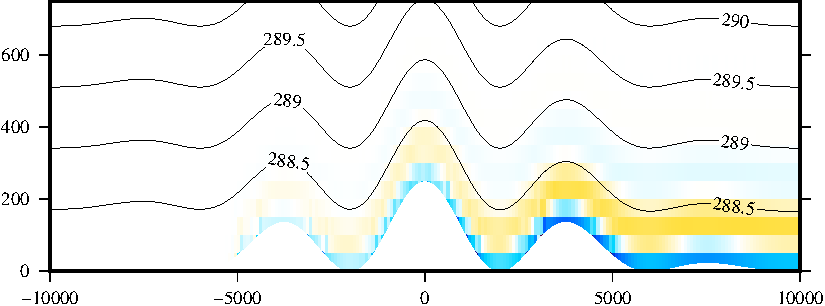
\includegraphics{tracerDiffMountain.pdf} \\
	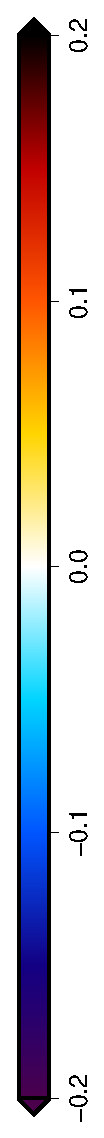
\includegraphics[height=5in,angle=270]{tracerDiffMountain_T_diff.eps}
%
	\caption{Error in tracer density in the thermal advection test at a resolution of $\Delta z = \SI{50}{\meter}$ on the cut cell grid.  Errors are generated near mountainous terrain and are advected horizontally on the lee side.  Contours in tracer density are overlayed.  Axes are in units of \si{\meter}.}
	\label{fig:tracerError}
\end{figure}

These new results led us to modify our original conclusion and instead we concur with the reviewer, finding that potential temperature errors in the mountain waves test are primarily due to numerical errors in the advection of potential temperature.

\subsection*{Cut cell grid generation}
\begin{figure}
	\centering
	\subcaptionbox{Cut cell grid with $\Delta z = \SI{250}{\meter}$.  Small cells next to the mountain peak have been merged with adjacent cells above. \label{fig:merged-cells}}[.48\linewidth]{\includegraphics[width=2.8in]{../gravityWaves-mesh-cutCell-250m-250dz/constant/mesh.pdf}}
	\subcaptionbox{Cut cell grid with $\Delta z = \SI{200}{\meter}$.  Thin cells are visible next to the mountain peak which remain long in the direction of flow. \label{fig:thin-cells}}[.48\linewidth]{\includegraphics[width=2.8in]{../gravityWaves-mesh-cutCell-250m-200dz/constant/mesh.pdf}}
%
	\caption{Example cut cell grids used in the mountain waves test with a peak mountain height of \SI{250}{\meter}, showing the central domain in the mountainous region.}
	\label{fig:cutCell-grids}
\end{figure}

Cut cell grids were generated using an off-the-shelf application to intersect a terrain surface with a uniform, rectangular grid.  The application includes heuristics that `snap' vertices to the terrain surface.
The technique results in grids that differ from the typical method as described by \citet{adcroft1997}.  Small cells are either merged with adjacent cells, as shown in figure~\ref{fig:merged-cells}, or thin cells are created such as those in figure~\ref{fig:thin-cells}.  In the latter case, thin cells remain long in the direction of the flow, and so they do not impose additional constraints on the Courant number.  

\section{Charney-Phillips staggering on arbitrary grids}
\label{sec:cp}
  We have spent a few weeks formulating a new scheme for arbitrary grids that is equivalent to Charney--Phillips staggering on uniform rectangular grids.  The prognostic thermodynamic variable, $b_f$, is a buoyancy-like quantity stored at cell faces such that $b_f = \theta_f \bm{\hat{g}}$ where $\theta_f$ is the potential temperature at the face and $\bm{\hat{g}}$ is the unit vector of gravitational acceleration.  On a uniform rectangular grid, this formulation reduces to a Charney--Phillips staggering with $b_f = 0$ on all vertically-oriented faces.  $\theta_f$ is currently transported in advective form using an explicit Eulerian second order scheme.  We identify necessary future work for this formulation in the following section.


\section{Future research}
We plan to further explore advection schemes for transporting temperature: to analyse the existing upwind-biased scheme on cut cell grids, and to develop new advection schemes for Charney--Phillips staggering on arbitrary grids.

\begin{description}
	\item[Upwind-biased advection for cut cell grids]{We have used the upwind-biased cubic advection scheme in a series of tests on cut cell grids.  Since MC1, we have improved the scheme to ensure that advection remains upwind-biased even when the downwind cell is very small.  This was necessary to maintain stability in different cut cell configurations and led to much smaller errors in all mountain waves tests.  The technique is currently implemented in OpenFOAM but is otherwise undocumented.  We should test variants of the advection scheme on cut cell grids to demonstrate the utility of this technique.  We will discuss the results of this work in a new journal article.
		
We will avoid the avoid the vertex-snapping heuristics previously used to generate cut cell grids, instead preferring a more straightforward grid generation method that still retains the long, thin cells from the old method.  The report will include a complete description of the new technique.}

\item[Thermal advection schemes on Charney--Phillips staggered arbitrary grids]{An overview of the new Charney--Phillips formulation was provided in section~\ref{sec:cp}.  We have performed some preliminary tests in OpenFOAM to establish that the scheme produces stable, realistic results.
		
\cite{arakawa-konor1996} presented vertical slice tests that exposed the unphysical behaviour of the Lorenz computational mode.  We will use these same tests to assess the behaviour of our Lorenz model, and to verify that the computational mode is not present in the Charney--Phillips formulation.
		
Further modifications to the scheme are expected to be necessary.  In particular, we believe that a more accurate advection scheme will be required.
Existing schemes are designed to advect temperature on grids that are fully-structured in the vertical and horizontal.  We intend to develop new schemes that are suitable for arbitrary grids with Charney--Phillips staggering.
The Met Office are keen for us to investigate Eulerian schemes for thermal advection, and our results will inform design decisions for their new Dynamo dynamical core.  We hope to compare our new advection schemes with the semi-Lagrangian scheme used in EndGame \citep{davies2005}.}
\end{description}

\subsection*{Additional future directions}
\begin{description}
	\item[Comparisons of existing results with Met Office models]{Following a meeting with the Met Office, we agreed that it might be valuable to compare our resting atmosphere and mountain waves test results with the vertical slice versions of EndGame or BLASIUS.}
	\item[Further mountain waves tests]{Following discussions at a workshop hosted by the Met Office, many were interested in potential advantages of alternative grid techniques over very steep orography.  Following \citet{yamazaki-satomura2010}, we could examine the numerical stability and accuracy of our model in 2D flow over semi-circular hills.  It was also suggested that flow of a neutrally stable atmosphere over orography would better reveal numerical errors.}
	\item[TF/cut cell blended grids]{
MC1 proposed blending elements of TF and cut cell techniques to create a new grid that performs well over high mountains and near steep mountains.
More recently, I have considered how new grid formulations might improve various mountain flows.  For example, a test might be constructed in which cold air runs down a slope pooling in a basin.  We might construct a grid that has high-resolution terrain-following layers along slopes and has cut cells in the basin.  Such a grid should improve accuracy of both advection-dominated and stagnant flows.

This research would be less directly useful to the Met Office since they intend to continue using TF grids.  Nevertheless, if we ensure that cells are aligned in columns then new types of grid might be implemented in Dynamo.}
\end{description}

\subsection*{Other research areas}
MC1 identified four further areas of research:
\begin{itemize}
	\item 3D tests on different grids to investigate flow blocking
	\item Large scale tests with Coriolis forces
	\item Mass coordinates with moving meshes to improve upper boundary treatment
	\item Modulating flow with resistance terms
\end{itemize}
We no longer intend to pursue these items: 3D and large-scale tests are not well-motivated by our current work, and we do not have a clear plan how we would improve on existing approaches which use mass coordinates. 

Also mentioned in MC1, Terry Davies put forward an idea for controlling sub-grid scale flow by adding a resistance term to the horizontal momentum equation.  We will not take this further because it involves designing heuristics for calculating coefficients and entails little numerical development.

Finally, {\citet{adcroft2013} described a technique for representing sub-grid scale bathymetry to model narrow channel flows in the ocean.  \citet{gohm2004} found that very high resolution was required to accurately model gap flows in the atmosphere, and so Adcroft's technique could be applied to the land to improve orographic flows at coarse resolutions.  We will not take this idea further because we would not be generating any new techniques ourselves.


\section{Training and development}

\subsection*{Taught modules}
In MC1, I had intended to enrol in several modules this year.  These decisions have changed as follows:
\begin{description}
\item[MA3NA2 Numerical Analysis II]{This module has been replaced with MA3NAT which spans two terms.  I would like to attend the second term which covers direct and iterative linear algebra solvers.  This will help me understand more about how matrix equations are solved in OpenFOAM and other atmospheric models.}
\item[MAMCDE Partial Differential Equations]{I will drop this module because I lack the prerequisite knowledge}
\item[MAMB10 Theory and Techniques of Data Assimilation]{I hope to attend Amos Lawless' Data Assimilation Short Course instead}
\end{description}
Finite elements are beginning to be used in atmospheric science and they are widely-used elsewhere, and so I might also consider taking M5MA47 Finite Elements in the spring.

\subsection*{Training}
I will be attending more RRDP modules this academic year:
\begin{description}
	\item[Open access for research publications]{}
	\item[Understanding the UK HE context]{Explains funding and assessment of university teaching and research}
	\item[IPR and copyright and intellectual property rights]{}
	\item[An essential guide to critical academic writing]{}
	\item[Preparing to teach]{This course will be mandatory for demonstrators as of September 2016}
\end{description}
I hope that the first three modules in particular will be helpful should I pursue a career in academia.

\subsection*{Conferences and presentations}
I attended the GungHo workshop on Next Generation Weather and Climate Prediction hosted by the Met Office in November 2015 and I was able to discuss my work with researchers in my field.  I also took the opportunity to meet with Met Office scientists afterwards to discuss my current and future work, and to experiment with the Dynamo codebase.  At an HHH meeting in October 2015, I presented what I've learnt about mountain meteorology and some of my ideas for future research.

\subsection*{Teaching and collaborations}
I was a teaching assistant for the NCAS Climate Modelling Summer School 2015, helping students implement linear advection and shallow water models.  This term, I am demonstrating for MTMG02 Atmospheric Physics.

I continue to collaborate with Hilary's intern, Yumeng Chen, who is investigating dimensionally-split, conservative advection schemes.  We have shared results of the \citet{schaer2002} tracer advection test and I hope to assist Yumeng in authoring a journal publication soon.

\bibliographystyle{ametsoc2014}                                                 
\bibliography{references}

\end{document}
